\documentclass[12pt,a4paper]{article}
\usepackage[utf8x]{inputenc}
\usepackage{ucs}
\usepackage[spanish]{babel}
\usepackage{amsmath}
\usepackage{amsfonts}
\usepackage{amssymb}
\usepackage{makeidx}
\usepackage{graphicx}
\usepackage{hyperref}
\usepackage{listings}
\usepackage{multicol}
\usepackage{float}
\hypersetup{
	colorlinks,
	citecolor=black,
	filecolor=black,
	linkcolor=red,
	urlcolor=black
}
\usepackage[width=17.00cm, height=23.00cm]{geometry}
\author{Jorge Yero Salazar - C412\\ Jose Diego Menendez Del Cueto - C412\\ Jose Ariel Romero Acosta - C412}
\title{Reporte de entrega del proyecto final de la
	asignatura Complementos de Compilación}
\date{Curso: 2018-2019}
\lstset{
	language=bash,
	breaklines=true,
	tabsize=1
}
\begin{document}
	\maketitle
	\tableofcontents
	\newpage
	\section{Introducción}
		En el presente reporte se tratan los aspectos fundamentales de la implementación de un compilador de COOL. En la sección 2 se plantean como obtener y utilizar el proyecto, se analizan todos los requerimientos y cual es la funcionalidad del compilador. La sección 3 expone cual es la arquitectura del compilador implementado, se plantean las diferentes fases desde que se recibe el código COOL hasta obtener el código ensamblador. En la sección 4 se trata sobre el analizador léxico y el sintáctico y la utilización de una herramienta generadora de analizadores lexicográficos y sintácticos así como las modificaciones que se le hizo a la gramática de COOL. La sección 5 trata sobre el analizador semántico cuales fueron las fases por las que se pasa y el por qué de ellas. La sección 6 sobre la generación de código intermedio, la explicación cual código fue utilizado que no es uno estandarizado sino uno definido por nosotros. La sección 7 sobre la generación de código ensamblador en cuyo caso la arquitectura es MIPS. En la sección 8 se trata una de las fases mas interesantes pues se trata la estrategia seguida para probar el compilador y se puede apreciar su funcionamiento.
	\section{Requisitos y uso del proyecto}
		La presente implementación de un compilador del lenguaje COOL fue echa en
		.Net Core 2.1. El único requisito para poder utilizar el compilador es tener instalado la versión 2.1 o superior. El proyecto puede ser descargado ejecutando 
		\begin{lstlisting}
			git clone https://github.com/matcom-compilers-2019/cool-compiler-supercool.git
		\end{lstlisting}
		y para conocer mas información acerca de los requerimientos y el uso debe leerse \url{https://github.com/matcom-compilers-2019/cool-compiler-supercool/doc/Readme.md}
	\section{Arquitectura}
		\begin{figure}[H]
			\centering
			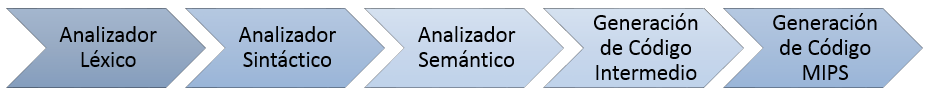
\includegraphics[scale=0.5]{Informe/Arquitectura.png}
			\caption{Arquitectura del compilador}
			\label{arch}
		\end{figure}
		La arquitectura de la presente implementación del compilador se puede observar en la figura \ref{arch}. El punto de entrada es el código de COOL, y las etapas quedarían como se muestra a continuación, la entrada de cada etapa es la salida de la etapa anterior, excepto en la primera que es el propio código COOL
		\begin{enumerate}
			\item \textbf{Analizador léxico:} El código COOL es procesado por un código generado automático por ANTLR4 a partir de la gramática de COOL definida, este devuelve como salida el \textbf{Syntax Tree(ST)}.
			\item \textbf{Analizador sintáctico:} Se hace uso del patrón visitor para a partir del ST construir el \textbf{Abstract Syntax Tree(AST)} y se construye la tabla de símbolos.
			\item \textbf{Analizador semántico:} Se hace uso del patrón visitor nuevamente esta vez con 3 recorridos sobre el AST donde se construyen los objetos, los métodos y se realiza el chequeo de tipos respectivamente.
			\item \textbf{Generación de código intermedio:} Se hace uso del patrón visitor para a partir del AST ya chequeado generar una especie de árbol que contiene nodos del intermediate language(IL) definido.
			\item  \textbf{Generación de código MIPS:} Se hace uso del patrón visitor para a partir de cada nodo del árbol de IL generar su correspondiente código MIPS.
		\end{enumerate}
		 
	\section{Analizador Léxico y Analizador Sintáctico}
		La implementación del tokenizer y del parser se realizaron con ANTLR4.Se especificaron las reglas del lexer y del parser tomando como base la especificada en el manual de COOL. Los Errores de lexer fueron detectados declarando un tipo de token especial que reconozca todas las palabras del lenguaje.
		
		El problema de la precedencia entre los operadores fue resulto haciendo uso de ANTLR ya que esta permite determinar prioridades entre las partes derechas de producciones que tengan la misma cabecera.	Otro problema resuelto con las facilidades de ANTLR4 fue el de la asociatividad a la derecha del operador de asignación, bastó con especificar su asociatividad en la producción correspondiente. Luego se hace uso de patrón visitor para construir un AST de COOL a partir del ST devuelto por ANTLR en el proceso de Parsing, en este momento se construye la tabla de símbolos, una estructura que representa al concepto de ámbito del lenguaje y permite determinar a partir de un string y un contexto el símbolo asociado.   
	\section{Analizador Semántico}
		Durante la fase de análisis semántico se realizan 3 recorridos usando también el patrón visitor los dos primeros para construir los contextos de objetos y de métodos respectivamente y una última corrida para realizar el chequeo de tipos. Durante la
		construcción de los contextos se detectan errores que no aparecen como parte de expresiones. 
		
		Un problema importante en esta etapa es detectar la mayor cantidad de errores posibles, de forma  tal que se evite un comportamiento en cascada. Para resolver este problema el chequeo se creo un tipo especial el \textbf{Null\_Type}, tipo sobre el cual todas las operaciones están definidas, si una expresión contiene un error semántico entonces se marca como incorrecta sin embrago el tipo asociado a la expresión es \textbf{Null\_Type} lo cual permite que no haya comportamiento en cascada a la hora de detectar los errores, ya que el padre del nodo revisado tendrá como hijo un nodo que devuelve \textbf{Null\_Type} sobre el cual todas las expresiones están bien definidas.
		
		Los errores que se detectan en una etapa son críticos en el análisis de la siguiente por eso no se avanza a la siguiente etapa si la actual falla por alguna razón.
		\subsection{Boxing y Unboxing}
			Uno de los aspectos fundamentales fue detectar en los lugares donde era necesario hacer boxing y unboxing.
			\begin{center}
				Lugares donde se hizo boxing 
			\end{center} 
			\begin{multicols}{2}
				\begin{itemize}
					\item paso de argumentos
					\item retorno de funciones de tipos por referencia
					\item distpatch
					\item expr0 en un case
				\end{itemize}
			\end{multicols}
			\begin{center}
				Lugares donde se hizo unboxing 
			\end{center} 
			\begin{multicols}{2}
				\begin{itemize}
					\item en las expresiones del case que fueran de tipos por valor
					\item después de haber ejecutado al copy de un tipo por valor
				\end{itemize}
			\end{multicols}
	\section{Generación de Código Intermedio}
		En la etapa de generación de código intermedio se generó a un código intermedio que no es está estandarizado sino a uno establecido por nosotros el cual estaba mas cercano a COOL que a ensamblador, esto nos limitó las cosas que se podían hacer en el código intermedio y en ocasiones se tuvo que generar código mips directamente de la salida del AST como en el caso de la expresión case, si el código intermedio generado por nosotros estuviese a un nivel mas bajo se podría haber resuelto esta expresión en esta etapa sin necesidad de bajarlo directamente a la próxima. Para la generación de código se realiza un visitor sobre el AST que da como salida el analizador semántico y se traducen los nodos del AST a uno o mas nodos de código intermedio, los nodos que se decidió bajar directamente del AST a la generación de código ensamblador lo que se realizó fue crear un nodo en esta etapa prácticamente con la misma signatura que en el AST y se asignaron sus parámetros.
	\section{Generación de Código MIPS}
		Para la generación del código ensamblador, en este caso el código mips lo que se realiza es un visitor sobre el árbol de codigo intermedio que se generó como se explicó en la sección anterior, luego se traduce cada nodo de código intermedio a código mips. Para facilitar esta etapa se realizo un Helper con macros implementadas que fueron de gran utilidad como 
		Push, Pop, Call, PrintInt, PrintString, Add, Sub, Mul, Div, entre otras.
		\subsection{Representación de tipos}
			Uno de los aspectos importantes a destacar es como se representaron los tipos en mips, para ello se dividen los tipos en tipos por valor y tipos por referencia. Los tipos por referencia son representados de la siguiente forma
			\begin{multicols}{2}
				\begin{table}[H]
					\centering
					\begin{tabular}{|c|c|}
						\hline
						índice & valor \\\hline
						-4 & type\_info \\\hline
						0 & atributo$_1$ \\\hline
						\vdots & \vdots \\\hline
						$4*(n-1)$ & atributo$_n$ \\\hline 
					\end{tabular} 
					\caption{Representación de un tipo por referencia}		
				\end{table}
				\begin{table}[H]
					\centering
					\begin{tabular}{|c|c|}
						\hline
						índice & valor \\\hline
						0 & type\_name\_ref \\\hline
						4 & allocate\_size \\\hline
						8 & virtua\_table\_ref \\\hline
					\end{tabular}
					\caption{Representación del type\_info}		
				\end{table}
			\end{multicols}
		\begin{table}[H]
			\centering
			\begin{tabular}{|c|c|}
				\hline
				índice & valor \\\hline
				0 & función$_1$\_ref \\\hline
				\vdots & \vdots \\\hline
				$4 * (n - 1)$ & función$_n$\_ref \\\hline
			\end{tabular}
			\caption{Representación de la virtual\_table}		
		\end{table}
	\section{Probar del compilador}
		El compilador viene con un conjunto de test para probar todas las funcionalidades, estos pueden probarse estando en la raíz del proyecto y ejecutando 
		\begin{lstlisting}
			make tests
		\end{lstlisting}
		los test solo son capaces de ejecutarse en Linux 64 bits y Windows 10 64 bits. Es necesario tener instalado spim para poder correr el código mips, en Windows 10 es necesario tener instalado \textit{Windows Subsystem For Linux}. Hay test que ejecutan hacen la ejecución completa del compilador, ademas ejecutan el código mips, para saber si la salida es correcta se compara utilizando ademas del compilador implementado otro compilador para y se comparan las salidas de ambos.
\end{document}